\begin{figure*}[t]
    \centering
    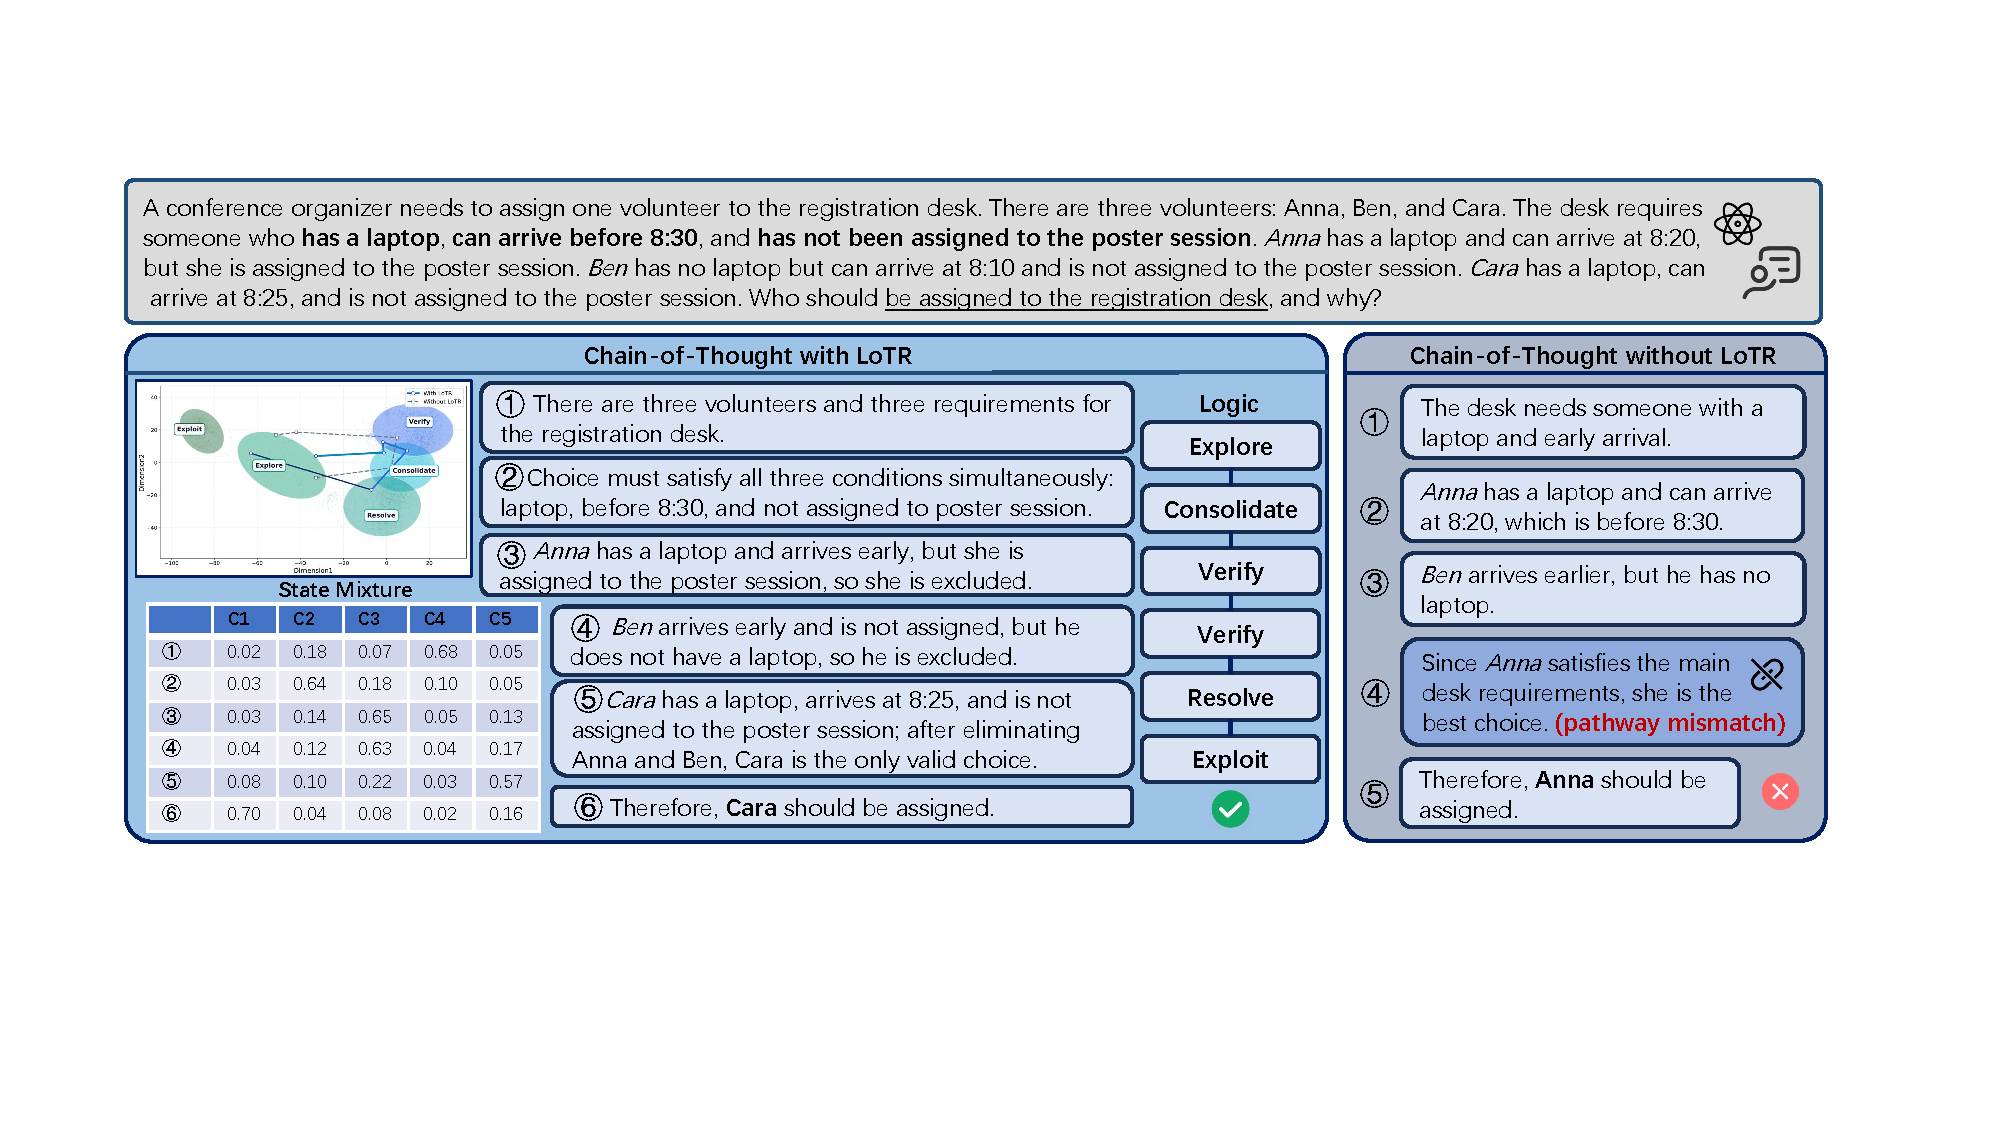
\includegraphics[width=\linewidth]{figs/lotr_case_study.pdf}
    \vspace{-4mm}
    \caption{\textbf{Qualitative case study.} Representative trajectory \emph{with} vs.\ \emph{without} LoTR under CoT.}
    \label{fig:lotr_case_study}
    \vspace{-5mm}
\end{figure*}

\vspace{-2mm}
\section{Related Work}
\label{sec:related}

\vspace{-1mm}
\paragraph{External reasoning paradigms for LLMs.}
A large body of work improves LLM reasoning by changing the \emph{external} procedure followed at inference time, including chain-of-thought prompting \citep{wei2022chain}, least-to-most decomposition \citep{zhou2023least}, plan-based prompting \citep{wang2023plan}, program-aided reasoning \citep{chen2023pot,gao2023pal}, iterative self-refinement \citep{madaan2023selfrefine}, self-consistency and sample aggregation \citep{lightman2024verify,wang2023selfconsistency}, best-of-$N$ sampling and test-time compute scaling \citep{brown2024llmmonkeys,chow2024inferenceaware,snell2025scaling}, and tree- or search-based reasoning \citep{xie2024mcts,yao2023tree,yao2023react}. These methods primarily prescribe a stronger trajectory-level scaffold or allocate more computation to sampling, branching, verification, or tool-like decomposition. LoTR is orthogonal to this direction: it keeps the external scaffold fixed and studies whether each reasoning step can be internally executed through a pathway matched to the logic state induced by that scaffold.
\vspace{-1mm}

\paragraph{Internal and latent structure of reasoning.}
Another line of work analyzes the internal organization of transformer computation, including attention-head specialization \citep{michel2019sixteen,voita2019analyzing}, induction heads and circuit-level mechanisms \citep{olsson2022induction}, and structured representation geometry in language models \citep{zou2023representationengineering}. Recent studies further suggest that reasoning is not internally uniform: hidden states may encode correctness or verification signals \citep{zhang2025reasoningmodels}, and multi-step trajectories can exhibit step-specific representation geometry \citep{sun2026trajectories}. Closely related latent-reasoning methods move reasoning into continuous hidden space rather than decoded token space \citep{hao2024coconut}. LoTR builds on the view that reasoning has structured latent states, but differs in purpose: it neither replaces language-level reasoning with a latent trajectory nor stops at interpretation. Instead, it turns recurring logic states into reusable control signals for routing internal computation under existing reasoning paradigms.
\vspace{-1mm}

\paragraph{Plug-in control and inference-time steering.}
LoTR is also related to frozen-model intervention methods, including inference-time intervention over selected heads \citep{li2023inference}, activation steering through additive latent directions \citep{rimsky2024caa,turner2024actadd}, and representation engineering approaches that manipulate behavior through latent directions \citep{zou2023representationengineering}. Recent reasoning-oriented steering methods further retrieve or compose latent steering signals during inference, such as STIR and RISER \citep{shi2026stir,ye2026riser}. These methods show that model behavior can be changed without weight updates, but their control objects are typically global directions, retrieved impulses, or routed steering vectors. LoTR instead uses a sentence-level mixture over recurring logic states to compose \emph{head-level pathway templates}, tying the intervention to the evolving logic of multi-step reasoning rather than to a fixed attribute direction or task-level steering.
\vspace{-1mm}

\paragraph{Probes and representation-based control.}
Probing methods use lightweight classifiers to read structured information from model representations \citep{alain2016understanding,belinkov2022probes}. In reasoning settings, probes have been used to expose hidden correctness or verification signals and to support decisions such as early stopping \citep{zhang2025reasoningmodels}. LoTR uses probes in a different role: the probe is not a final verifier or post-hoc interpreter, but an online estimator of logic-state activations. These activations are mapped to a reusable routing policy over head-level pathway templates. Thus, LoTR turns representation readout into reasoning-time control: latent states are not only measured, but used to determine how the next reasoning step is internally realized.
\vspace{-1mm}